\documentclass{article}

% Language setting
% Replace `english' with e.g. `spanish' to change the document language
\usepackage[english]{babel}

% Set page size and margins
% Replace `letterpaper' with `a4paper' for UK/EU standard size
\usepackage[letterpaper,top=2cm,bottom=2cm,left=3cm,right=3cm,marginparwidth=1.75cm]{geometry}

% Useful packages
\usepackage{amsmath}
\usepackage{graphicx}
\usepackage[colorlinks=true, allcolors=blue]{hyperref}
\usepackage{listings}

\usepackage[style=authoryear-ibid,backend=biber]{biblatex}

\usepackage{xcolor}

\usepackage{csquotes}% Recommended
\addbibresource{projectreport.bib}% Syntax for version >= 1.2

\definecolor{codegreen}{rgb}{0,0.6,0}
\definecolor{codegray}{rgb}{0.5,0.5,0.5}
\definecolor{codepurple}{rgb}{0.58,0,0.82}
\definecolor{backcolour}{rgb}{0.95,0.95,0.92}

\lstdefinestyle{pythonstyle}{
    backgroundcolor=\color{backcolour},   
    commentstyle=\color{codegreen},
    keywordstyle=\color{magenta},
    numberstyle=\tiny\color{codegray},
    stringstyle=\color{codepurple},
    basicstyle=\ttfamily\footnotesize,
    breakatwhitespace=false,         
    breaklines=true,                 
    captionpos=b,                    
    keepspaces=true,                 
    numbers=left,                    
    numbersep=5pt,                  
    showspaces=false,                
    showstringspaces=false,
    showtabs=false,                  
    tabsize=2
}

\lstset{style=pythonstyle}

\begin{document}

\begin{titlepage}
    \begin{center}
        \vspace*{1cm}
        \LARGE\textbf{CCT College Dublin}\\
        \vspace{0.5cm}
        \Large Assessment Cover Page\\
        \hrulefill\\
        \vspace{1cm}
        \begin{tabular}{|l|p{7cm}|}
        
        \hline
        Module Title:& Strategy Thinking \\
        \hline
        Assessment Title:& Project Report\\
        \hline
        Lecturer Name:& James Garza\\
        \hline
        Student Full Name:& Giulio Calef, Kevin Byrne and Victor Ferreira Silva \\
        \hline
        Student Number:& sba22314, sba22264, 2021324 \\
        \hline
        Assessment Due Date:& 7th May 2023\\
        \hline
        Date of Submission:& 7th May 2023\\
        \hline
        \end{tabular}
        
        \vspace{1cm}
        \Large Declaration\\
        \vspace{0.5cm}
        \normalsize By submitting this assessment, I confirm that I have read the CCT policy on Academic Misconduct and understand the implications of submitting work that is not my own or does not appropriately reference material taken from a third party or other source. I declare it to be my own work and that all material from third parties has been appropriately referenced. I further confirm that this work has not previously been submitted for assessment by myself or someone else in CCT College Dublin or any other higher education institution.\\
    \end{center}
\end{titlepage}



\begin{titlepage}
   \begin{center}
       \vspace*{1cm}

       \textbf{Detecting and Predicting Severe Slugging in Petrobras 3W Data Set}

       \vspace{0.5cm}
        Strategic Thinking Capstone Project
            
       \vspace{1.5cm}

       \textbf{Giulio Calef} \\
       \textbf{Kevin Byrne} \\
       \textbf{Victor Ferreira Silva} \\

       \vfill
            
       Strategic Thinking Capstone Project
            
       \vspace{0.8cm}
     
       % \includegraphics[width=0.4\textwidth]{university}
            
       Higher Diploma in Science in Artificial Intelligence Applications\\
       CCT College Dublin\\
       Ireland\\
       May 2023
            
   \end{center}
\end{titlepage}

\title{Detecting and Predicting Severe Slugging in Petrobras 3W Data Set}

\author{Giulio Calef, Kevin Byrne, Victor Ferreira Silva}
\tableofcontents

\maketitle

\section{Introduction}

Operational safety, productivity, quality are general key objectives in any industry, and in the oil and gas industry, environmental concerns are not only crucial, but they also pose as an immense daily challenge. 

Generally, the oil industry has been increasingly adopting automated controls and monitoring processes \parencite{venkatasubramanian_rengaswamy_yin_kavuri_2003} to comply with the increasingly higher standards in their operations. Such standards not only require more productive operations, but safer processes and more energy-efficient methods to achieve greater quality \parencite{jounela_2007}.

Thus, any event which can cause a production loss in an oil field are certainly very costly, in pure economic terms, but can also have dire costs in terms of human lives and of damage to our environment that can be hard to address or almost permanent in some cases. Therefore, any technique that can help early detection and/or prevention of technical accidents in the oil industry is therefore very welcome and “worth as gold”. 

Offshore oil wells provide some of the most challenging operating conditions in the industry, with additional complexity due to the peculiarities of operating at sea and the limited amount of instrumentation that can be deployed to monitor and control the well operational status.

One of the main challenges in oil industry is predicting undesirable events such as \emph{Severe Slugging}. Severe Slugging is an critical flow assurance issue, commonly observed in offshore pipeline-riser systems, documented for the first time by \textcite{yocum_1973}. Some of the consequences of this issue include flooding of downstream production facilities and an overall decrease in productivity. According \textcite{revvargas2019} depending on the frequency it occurs and intensity, this event may even damage the equipment in the well, although specific operational actions can be taken to mitigate this issue since it is detected.

According \textcite{revvargas2019}, a simplified description of a typical offshore well can be seen in Figure \ref{fig:offshore_well} and its structure is basically composed by:

\begin{itemize}
\item The Christmas Tree, a structure lying on the seabed, at the well head, with pressure and temperature sensors and safety valves
\item An Electro-Hydraylic Umbilical, which is how The Christmas Tree is remotely controlled.
\item The Permanent Downhole Gauge (PDG), installed at the Christmas Tree;
\item The Temperature and Pressure Transducer (TPT), also a part of the Christmas Tree;
\item The Production Choke (PCK), installed on the drilling vessel/rig at the top;
\item The Downhole Safety Valve (DHSV), a safety valve installed in the production tubing of wells
\end{itemize}


\begin{figure}
\centering
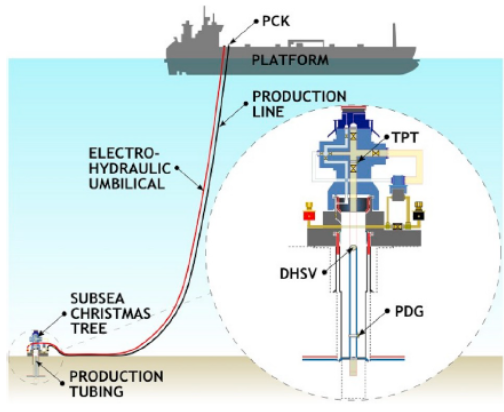
\includegraphics[width=0.6\textwidth]{offshore_well.png}
\caption{\label{fig:offshore_well}Schematic of a typical offshore well}
\end{figure}

Given this, Petrobras, the Brazilian oil company, has developed a data set (3W) that contains data for the most common monitored variables in offshore oil wells. This project aims to understand the relations between these variables and oil well operational anomalies, such as Severe Slugging.

\subsection{Hypothesis}
The data present in 3W Data Set allows classifier models to predict Severe Slugging with high accuracy.

\subsection{General Goal}
The business objective of our project is to apply machine learning techniques modeled in this project to the 3W data set to accurately predict \emph{Severe Slugging} in an offshore well production line. Achieving a significant accuracy in these predictions should be possible by identifying the correlations between the variables presented in the records monitored in an offshore oil well operation. 


\subsection{Success Criteria}
Success will be defined as the ability to accurately predict one or more of the conditions leading to an undesirable event. Given the potentially catastrophic impacts (ethical, environmental, economic) of accidents in the oil industry, the ability to predict a potential risk so that a quick reaction/fix can avoid unrecoverable conditions has a clear business value.

\subsection{Methodologies and Technologies}

The methodology that guided the iterations this project was CRISP-DM. Given this, a number of libraries were used throughout this process to support most of its distinct stages, that is, Data Understanding, Data Preparation, Modeling, and Evaluation. 

Once the methodology was defined, Petrobras' \emph{3W Tool Kit} was studied and used to extract the data from the instances interesting to the project, that is, from the real instances that effectively presented the Severe Slugging event.

Then, \emph{Pandas} and \emph{NumPy} libraries were selected for data manipulation and analysis. Then, the base machine learning library for the majority of models in this project was \emph{Scikit-learn}, as it offers various preprocessing, classification models and clustering algorithms. Another library imported in this project was \emph{Keras}, which is is an open-source solution that provides an interface for artificial neural networks.

Besides that, \emph{StandardScaler} from the \emph{Scikit-learn} library was selected for scaling and normalisation of the data. Given the high data imbalance presented by the data set, a \emph{RandomUnderSampler} was also from \emph{Imbalanced-learn} library was imported. Regarding feature reduction, the decomposition algorithm \emph{PCA}, also from \emph{Scikit-learn}, was adopted here in this study. 

Also, \emph{Seaborn}, \emph{Matplotlib} and \emph{Plotly} libraries were widely used to analyse data throughout the project and provide data visualisation using at the Evaluation stage. Another tool from \emph{Scikit-learn} selected as a baseline model was \emph{DummyClassifier}. 

Additionally, the following tools from module \emph{model\_selection} in \emph{Scikit-learn} library were chose:

\begin{itemize}
    \item \emph{GridSearchCV}, for hyperparameter tuning
    \item \emph{cross\_val\_score} for cross-validation, 
    \item \emph{train\_test\_split} for train/test splitting,
    \item \emph{KFold} for cross-validation during Evaluation
\end{itemize}

Ultimately, \emph{Scikit-learn} library also provided the following classifiers for this project:
\begin{itemize}
    \item LinearSVC, from \emph{svm} module,
    \item KNeighborsClassifier, from \emph{neighbors} module,
    \item DecisionTreeClassifier, from \emph{tree} module,
    \item RandomForestClassifier, from \emph{ensemble} module
\end{itemize}

Lastly, the modules \emph{make\_pipeline} and \emph{Pipeline} from \emph{Scikit-learn} were used to chain all steps of the workflow together, and the library \emph{Pickle} was selected to persist the resulting models in file.


\subsection{Accomplishment}
After extracting using 3W Tool Kit and some CRISP-DM iterations, this project presented 2 models with a high accuracy.

\section{Data Understanding}

Pre-processing a data set through data characterisation involves summarising the features and characteristics present in the data using statistical measures and visualisations techniques such as bar charts and scatter plots. After this stage, it should be possible to identify biases, patterns, trends, and any missing or irrelevant data in the data set that may need to be addressed.

This data set is composed by instances of eight types of undesirable events characterized by eight process variables from three different sources: real instances, simulated instances and hand-drawn instances. All real instances were taken from the plant information system that is used to monitor the industrial processes at an operational unit in Brazilian state of Espírito Santo. The simulated instances were all generated using OLGA, a dynamic multi-phase flow simulator that is widely used by oil companies worldwide \parencite{andreolli2016introduccao}. Finally, the hand-drawn instances were generated by a specific tool developed by Petrobras researchers for this data set to incorporate undesirable events classified as rare.

Ultimately, only the data from the real instances was selected for this project, as simulated instances and hand-drawn instances did not present any record for two features relevant to Severe Slugging, namely Gas Lift Flow Rate and Pressure Variable Upstream Of the Gas Lift Choke.

\subsection{Data Collection}
The data used in this study was extracted after following the documentation from 3W took kit \parencite{petrobras3WToolkit}, which is a Python software package with resources to experiment machine learning-based approaches and algorithms for issues related to undesirable events. The specific data used in this study was from the \emph{real instances}, and it was also available at \textcite{extracted3Wcsv} at the time of publication of this study.

\subsection{Data Characterisation}

The selected data set consists of 13,952,911 observations, with 14 columns of data for each observation. The first column, label, indicates the event type for each observation. The second column, well, contains the name of the well the observation was taken from. Hand-drawn and simulated instances have fixed names for in this column, while real instances have names masked with incremental id. The third column, id, is an identifier for the observation and it is incremental for hand-drawn and simulated instances, while each real instance has an id generated from its first timestamp. The columns representing the process variables are:



The pressure features are measured in Pascal (Pa), the volumetric flow rate features are measured in standard cubic meters per second (SCM/s), and the temperature features are measured in degrees Celsius (°C).

Other information are also loaded into each pandas Dataframe:

\begin{itemize}
\item label: instance label (event type) - target variable;
\item well: well name. Hand-drawn and simulated instances have fixed names (respectively, drawn and simulated. Real instances have names masked with incremental id;
\item id: instance identifier. Hand-drawn and simulated instances have incremental id. Each real instance has an id generated from its first timestamp;
\item class: Although it can be used to identify periods of normal operation, fault transients, and faulty steady states, which can help with diagnosis and maintenance, it is a category which results from label, which is our target here
\end{itemize}



In order to maintain the realistic aspects of the data, the data set was built without pre-processing, including the presence of NaN values, frozen variables due to sensor or communication issues, instances with varying sizes, and outliers \parencite{revvargas2019}.

A concise summary of this data set generated by \emph{pandas.DataFrame.info} method can be seen on Table ~\ref{tab:widgets}.

\begin{table}
\centering
\begin{tabular}{l|r|r}

Column & pandas.Dtype & Description\\\hline
timestamp & datetime64[ns] & timestamp \\
label & int64 & label \\        
well & object & well \\       
id & int64 & id \\        
P-PDG & float64 & pressure variable at the PDG, in Pa \\      
P-TPT & float64 & pressure variable at the TPT, in Pa \\     
T-TPT & float64 & temperature variable at the TPT, in °C \\      
P-MON-CKP & float64 & pressure variable upstream of CKP, in Pa \\      
T-JUS-CKP & float64 & temperature variable downstream of CKP, in °C \\      
P-JUS-CKGL & float64 & pressure variable upstream of CKGL, in °C \\       
T-JUS-CKGL & float64 & temperature variable upstream of CKGL,  in °C\\     
QGL & float64 & gas life flow rate, SCM/s\\      
class & float64 & operation state: normal, fault, faulty steady \\   
source & object & type of instance: real, simulated or hand-drawn \\     

\end{tabular}
\caption{\label{tab:widgets}Summary of the data set compiled from real instances}
\end{table}


The labels are:

\begin{itemize}
\item 0 - Normal Operation = Normal
\item 1 - Abrupt Increase of BSW = AbrIncrBSW
\item 2 - Spurious Closure of DHSV = SpurClosDHSW
\item 3 - Severe Slugging = SevSlug
\item 4 - Flow Instability = FlowInst
\item 5 - Rapid Productivity Loss = RProdLoss
\item 6 - Quick Restriction in PCK = QuiRestrPCK
\item 7 - Scaling in PCK = ScalingPCK
\item 8 - Hydrate in Production Line = HydrProdLine
\end{itemize}

\subsection{Exploratory Data Analysis}

A bar chart was generated displaying the percentage of present values in each column of the data frame - see Figure \ref{fig:missingvalues}. The data set contained missing values in several columns, thus some columns and row were deleted in order to obtain accurate and reliable results.

Three boxplots were plotted to show how the data was distributed before any data cleaning - see Figure \ref{fig:distr_boxplots_before_cleaning}. They were divided according the feature measurement unit: the pressure features were measured in Pascal (Pa), the temperature features are measured in degrees Celsius (°C) and one feature about volumetric flow rate which was measured in standard cubic meters per second (SCM/s).

\begin{figure}
\centering
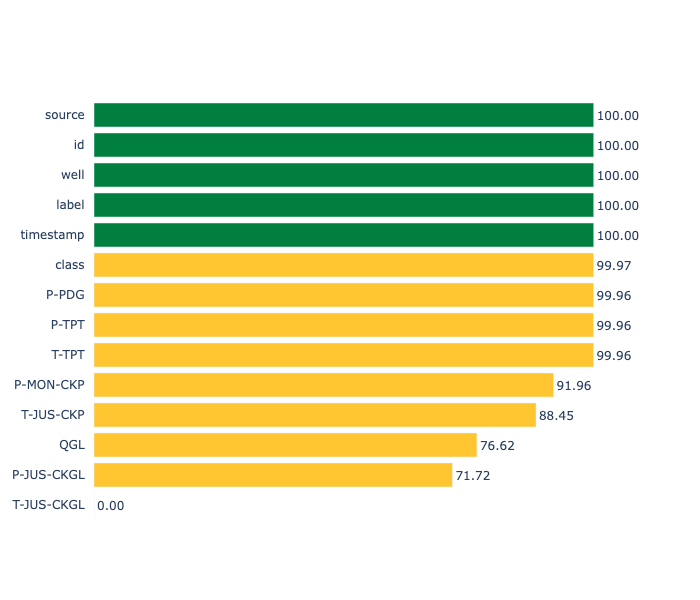
\includegraphics[width=1\textwidth]{missingvalues.png}
\caption{\label{fig:missingvalues}Proportion of available data per column, in \%.}
\end{figure}


\begin{figure}
\centering
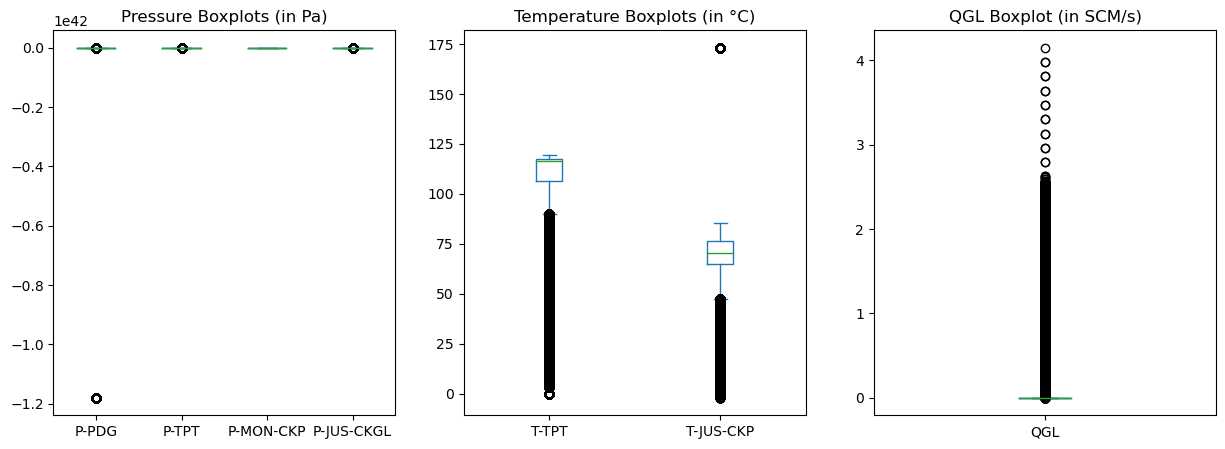
\includegraphics[width=1\textwidth]{distr_boxplots_before_cleaning.png}
\caption{\label{fig:distr_boxplots_before_cleaning}Box plots showing the distribution of pressure, temperature, and QGL (SCM/s) data for a set of oil wells.}
\end{figure}


\section{Data Preparation}

Data preparation included Data Cleaning, Feature Engineering, Train/Test Splitting and Handling Imbalanced Data, Data Scaling, and an analysis of the chosen approach regarding dimensionality reduction for some models.

\subsection{Data Cleaning}

The missing data from the following columns were removed: class, P-PDG, P-TPT, T-JUS-CKP, P-MON-CKP,T-TPT, P-MON-CKP, QGL and P-JUS-CKGL. After this, the columns class, T-JUS-CKGL (an empty column), id, source were dropped. Column class is a column which brings more details about label. Consider that columns timestamp, label were kept at this stage. Finally all duplicates were removed. 

\begin{lstlisting}[language=Python]
# dropping rows with missing or null class column
df_clean = df.dropna(subset=[
    'class','P-PDG','P-TPT','T-JUS-CKP','P-MON-CKP','T-TPT',
    'P-MON-CKP','QGL','P-JUS-CKGL'
])

# removing redundant columns
df_clean = df_clean.drop(['class','T-JUS-CKGL','id','source'], axis=1)

# checking duplicated rows after removing ids
df_clean = df_clean.drop_duplicates()

df_clean.info()
\end{lstlisting}

\begin{verbatim}
<class 'pandas.core.frame.DataFrame'>
Int64Index: 10003580 entries, 0 to 13952910
Data columns (total 10 columns):
 #   Column      Dtype         
---  ------      -----         
 0   timestamp   datetime64[ns]
 1   label       int64         
 2   well        object        
 3   P-PDG       float64       
 4   P-TPT       float64       
 5   T-TPT       float64       
 6   P-MON-CKP   float64       
 7   T-JUS-CKP   float64       
 8   P-JUS-CKGL  float64       
 9   QGL         float64       
dtypes: datetime64[ns](1), float64(7), int64(1), object(1)
memory usage: 839.5+ MB
\end{verbatim}

Also, as it can be seen on Figure \ref{fig:distr_boxplots_before_cleaning}, features P-PDG and P-TPT had the presence of extreme outliers. These outliers were also removed with the following code:

\begin{lstlisting}[language=Python]
# removing extreme outliers from P-PDG 
Q1 = df_clean['P-PDG'].quantile(0.25)
Q3 = df_clean['P-PDG'].quantile(0.75)
IQR = Q3 - Q1
lower_bound = Q1 - (3 * IQR)
df_no_outliers = df_clean[(df_clean['P-PDG'] >= lower_bound)]

# removing extreme outliers from P-TPT
Q1 = df_no_outliers['P-TPT'].quantile(0.25)
Q3 = df_no_outliers['P-TPT'].quantile(0.75)
IQR = Q3 - Q1
upper_bound = Q3 + (3 * IQR)
df_no_outliers = df_no_outliers[(df_no_outliers['P-TPT'] <= upper_bound)]

df_no_outliers.shape
\end{lstlisting}
\begin{verbatim}
(9780901, 10)
\end{verbatim}

These rows with presence of extreme outliers represented 2.26\% of the resulting rows so far. As a result the distribution of values in P-PDG and P-TPT were modified, as Figure \ref{fig:distr_boxplots_after_cleaning} shows.

\begin{figure}
\centering
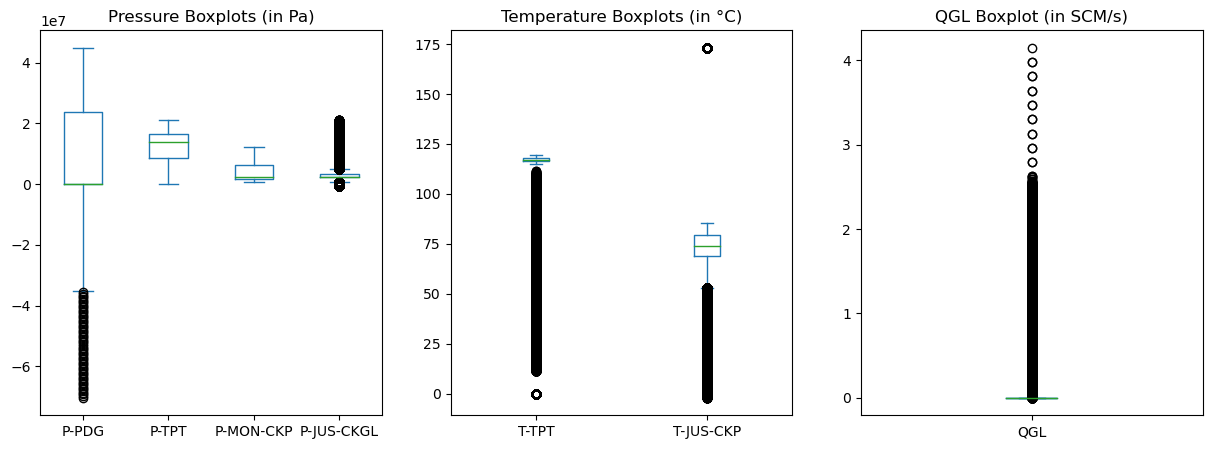
\includegraphics[width=1\textwidth]{distr_boxplots_after_cleaning.png}
\caption{\label{fig:distr_boxplots_after_cleaning}Box plots showing the distribution of pressure, temperature, and QGL (SCM/s) data without extreme outliers.}
\end{figure}


\subsection{Feature Engineering}

Given the label feature contains 8 possible numeric labels for each undesirable event and 1 label value 0 for normal observations, 8 new boolean columns were created for each one undesirable event, including for Severe Slugging, which is this project's target.

\begin{lstlisting}[language=Python]
dt_feat = df_no_outliers

# Changing 'label' column to object dtype
dt_feat['label'] = dt_feat['label'].astype('object') 

# Creating uint8 columns for each label
label_dummies = pd.get_dummies(dt_feat['label'], prefix='label')
dt_feat = pd.concat([dt_feat, label_dummies], axis=1)

# Renaming uint8 columns
column_names = {
    'label_0': 'Normal',
    'label_1': 'AbrIncrBSW',
    'label_2': 'SpurClosDHSW',
    'label_3': 'SevSlug', # target
    'label_4': 'FlowInst',
    'label_5': 'RProdLoss',
    'label_6': 'QuiRestrPCK',
    'label_7': 'ScalingPCK',
    'label_8': 'HydrProdLine'
}
dt_feat = dt_feat.rename(columns=column_names)

# Dropping the original 'label' column and Normal column, 
# since all other events must be 0
dt_feat = dt_feat.drop(['label','Normal'], axis=1)
dt_feat.info()
\end{lstlisting}
\begin{verbatim}
<class 'pandas.core.frame.DataFrame'>
Int64Index: 9780901 entries, 0 to 13952910
Data columns (total 16 columns):
 #   Column        Dtype         
---  ------        -----         
 0   timestamp     datetime64[ns]
 1   well          object        
 2   P-PDG         float64       
 3   P-TPT         float64       
 4   T-TPT         float64       
 5   P-MON-CKP     float64       
 6   T-JUS-CKP     float64       
 7   P-JUS-CKGL    float64       
 8   QGL           float64       
 9   AbrIncrBSW    uint8         
 10  SpurClosDHSW  uint8         
 11  SevSlug       uint8         
 12  FlowInst      uint8         
 13  RProdLoss     uint8         
 14  QuiRestrPCK   uint8         
 15  ScalingPCK    uint8         
dtypes: datetime64[ns](1), float64(7), object(1), uint8(7)
memory usage: 811.5+ MB
\end{verbatim}

Then all undesirable events columns were deleted but the column which denotes the observations presents Severe Slugging. The column \emph{HydrProdLine} concerned to Hydrate in Production line, however this event was not found in the data set resulting from real instances.

\begin{lstlisting}[language=Python]
dt_feat_target = dt_feat.drop([
#     , 'SevSlug', 'HydrProdLine',
    'AbrIncrBSW','SpurClosDHSW','FlowInst','RProdLoss','QuiRestrPCK','ScalingPCK'
], axis=1)

dt_feat_target.info()
\end{lstlisting}
\begin{verbatim}
<class 'pandas.core.frame.DataFrame'>
Int64Index: 9780901 entries, 0 to 13952910
Data columns (total 10 columns):
 #   Column      Dtype         
---  ------      -----         
 0   timestamp   datetime64[ns]
 1   well        object        
 2   P-PDG       float64       
 3   P-TPT       float64       
 4   T-TPT       float64       
 5   P-MON-CKP   float64       
 6   T-JUS-CKP   float64       
 7   P-JUS-CKGL  float64       
 8   QGL         float64       
 9   SevSlug     uint8         
dtypes: datetime64[ns](1), float64(7), object(1), uint8(1)
memory usage: 755.6+ MB
\end{verbatim}

\subsection{Train/Test Splitting}

The following code defined how the data set was split in Train and Test data sets. Additionally, the columns \emph{timestamp} and \emph{well} were removed and at the end the  distribution of the records according the presence or absence of Severe Slugging was computed.

\begin{lstlisting}[language=Python]
# defining features (X) and label (y)
target = 'SevSlug'

X = dt_feat_target.drop([target,'timestamp','well'], axis=1)
y = dt_feat_target[target]

# splitting data into train and test sets
X_train_u, X_test, y_train_u, y_test = train_test_split(X, y, test_size=0.3, random_state=42)

class_names = {0:'Non Sev Slug', 1:'SEV SLUGGING'}
print(y_train_u.value_counts(normalize=True).rename(index=class_names))
\end{lstlisting}
\begin{verbatim}
Non Sev Slug    0.94194
SEV SLUGGING    0.05806
Name: SevSlug, dtype: float64
\end{verbatim}

After the splitting process, the training data set had 6,846,630 rows and the test data set had 2,934,271 rows.

\subsection{Handling Imbalanced Data}

A \emph{RandomUnderSampler} was chosen to balance training data. As a result 50\% of observations presented Severe Slugging while the other 50\% were normal or presented other undesirable event. Test data set was not balanced since this project aim to best represent your deployment scenarios in real life.

\begin{lstlisting}[language=Python]
# balancing data 
balancing = RandomUnderSampler(random_state=42)

X_train, y_train = balancing.fit_resample(X_train_u, y_train_u)

class_names = {0:'Non Sev Slug', 1:'SEV SLUGGING'}
print(y_train.value_counts(normalize=True).rename(index=class_names))
print([X_train.shape, y_train.shape])
\end{lstlisting}
\begin{verbatim}
Non Sev Slug    0.5
SEV SLUGGING    0.5
Name: SevSlug, dtype: float64
[(795026, 7), (795026,)]
\end{verbatim}

Handling data imbalance is also important because it affects correlations - see as Figure \ref{fig:correlations} shows.

\begin{figure}
\centering
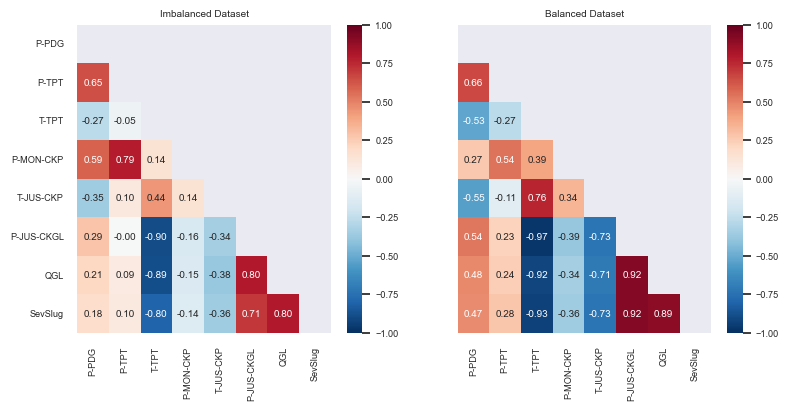
\includegraphics[width=1\textwidth]{correlations.png}
\caption{\label{fig:correlations}Correlations between variables before and after data balancing}
\end{figure}

\subsection{Data Scaling}

Although there are features presenting non-normal distributions, \emph{StandardScaler} was chosen as data scaler. It was chose because there are some features with strong correlation with Severe Slugging and lognormal distributions such as \emph{QGL} and \emph{P-JUS-CKGL} and as it is a method sensitive to the presence of outliers. The results of this transformation can be seen on Figure \ref{fig:std_scaler}.

\begin{figure}
\centering
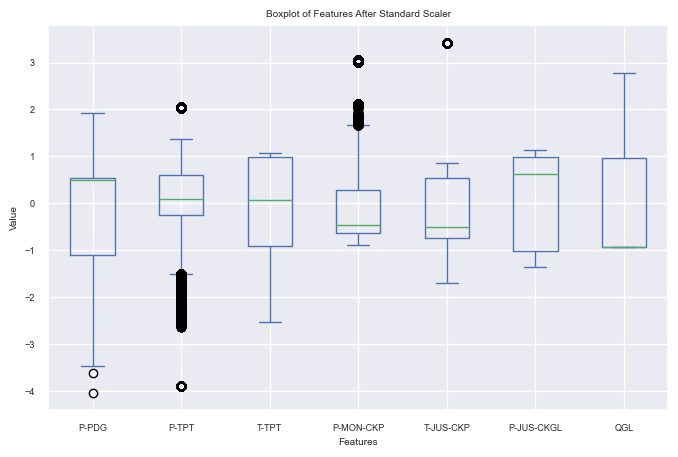
\includegraphics[width=1\textwidth]{std_scaler.png}
\caption{\label{fig:std_scaler}Box plot showing the distribution of the features in the training set after applying the StandardScaler transformation}
\end{figure}


\subsection{Dimensionality Reduction}

The unsupervised learning technique Principal Component Analysis (PCA) was chosen not only to prepare the data for some of the models studied here, but also to evidence any possible linear separability in this model. In Figure \ref{fig:pca} the results of this dimensionality reduction can be seen in two ways, with 2 and 3 components, although this process was unnecessary for the most successful models, that is, the non-linear classifiers.

\begin{figure}
\centering
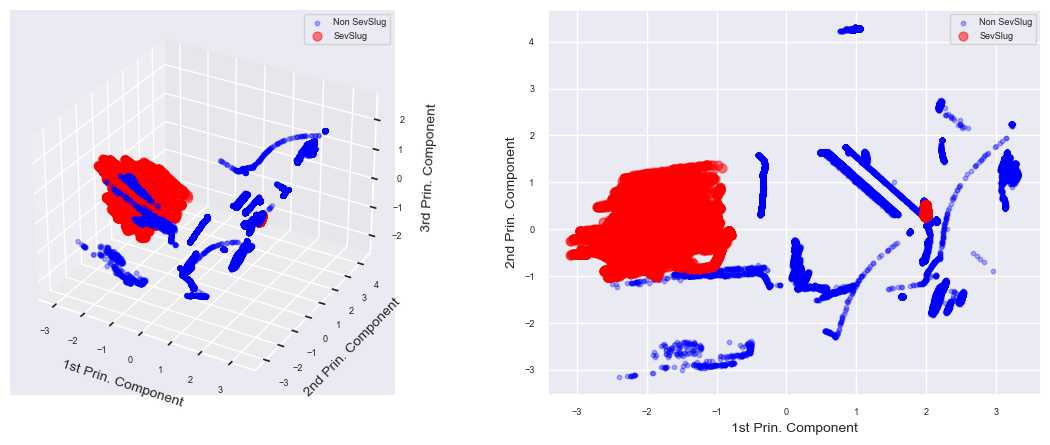
\includegraphics[width=1\textwidth]{pca.png}
\caption{\label{fig:pca}Visualisation of PCA applied to the data set showing a scatter plot for two (2D) and three (3D) principal components.}
\end{figure}

\section{Modeling}

For this project, five models were chosen: LinearSVC, k-Nearest Neighbors Classifier, Artificial Neural Network, Decision Tree Classifier and Random Forest Classifier. 

\subsection{Baseline: DummyClassifier}
Before proceeding with other models, a DummyClassifier was adopted to find a baseline for validation accuracy using the test data set. Given the distribution of the target variable in test data set, the baseline for any model was set in 94.17\%.

\begin{lstlisting}[language=Python]
dummy_pipeline = make_pipeline(StandardScaler(), DummyClassifier())
dummy_pipeline.fit(X_train, y_train)

# confirming score for Dummy classifier results from a balanced dataset
score = dummy_pipeline.score(X_train, y_train)

# predicting
y_predicted = dummy_pipeline.predict(X_test)
baseline = metrics.accuracy_score(y_test, y_predicted)

print("Score: ", score)
print("Accuracy: ",baseline)
\end{lstlisting}
\begin{verbatim}
Score:  0.5
Accuracy:  0.9417780429960286
\end{verbatim}

\subsection{LinearSVC}
Although the data is not linearly separable and it's not possible to find a condition of 100\% correctly classified by a hyperplane, a linear support vector classifier (LinearSVC) was implemented as part of this benchmark.

\subsubsection{Hyperparameter optimisation}
For finding the best parameters for this model, the hyperparameters to tune PCA and the model were specified. Then a pipeline was created with 3 steps:
\begin{enumerate}
\item \emph{scaler} which uses StandardScaler method to scale the data
\item \emph{dimred} which applies PCA dimensionality reduction
\item \emph{linearsvc} which applies the LinearSVC model.
\end{enumerate}

Finally, a grid search was performed using the above-mentioned pipeline and the hyperparameter grid to find the combination with the best accuracy metric with the default cross-validation, that is, a 5-fold cross-validation.
\begin{lstlisting}[language=Python]
from sklearn.svm import LinearSVC

param_grid = {
    'dimred__n_components': [3, 4], 
    'linearsvc__C': [1e-2, 1e-1, 1, 10, 100],
    'linearsvc__penalty':['l1', 'l2'],
    'linearsvc__dual': [False, True],
    'linearsvc__class_weight': ['balanced', None]
}

linear_svc_pipeline = Pipeline([
    ('scaler', scaler_pipeline), 
    ('dimred', PCA()), 
    ('linearsvc', LinearSVC())
])

grid_search_lsvc = GridSearchCV(
    linear_svc_pipeline,
    param_grid=param_grid,
    n_jobs=-1,
    scoring='accuracy',
    verbose=1
)

grid_search_lsvc.fit(X_train, y_train)
\end{lstlisting}

After this, the pipeline was defined with the best parameters found:
\begin{enumerate}
    \item StandardScaler()
    \item PCA(n\_components=3)
    \item LinearSVC(C=0.01, class\_weight='balanced', dual=False, penalty='l1')
\end{enumerate}

\subsubsection{Model training}
Then the model was trained using a similar pipeline, but this time with the optimal combination of parameters.

\begin{lstlisting}[language=Python]
linear_svc_pipeline = Pipeline([
    ('scaler', scaler_pipeline), 
    ('dimred', PCA(
        n_components=grid_search_lsvc.best_params_['dimred__n_components']
    )),
    ('linearsvc', LinearSVC(
        dual=grid_search_lsvc.best_params_['linearsvc__dual'],
        C=grid_search_lsvc.best_params_['linearsvc__C'],
        penalty=grid_search_lsvc.best_params_['linearsvc__penalty'],
        class_weight=grid_search_lsvc.best_params_['linearsvc__class_weight']
    ))
])

linear_svc_pipeline.fit(X_train, y_train)
\end{lstlisting}

\subsection{k-Nearest Neighbors Classifier}
A k-Nearest Neighbors Classifier (KNeighborsClassifier) was implemented as part of this benchmark.

\subsubsection{Hyperparameter optimisation}
For finding the best parameters for this model, the hyperparameters to tune PCA and the model were specified. Then a pipeline was created with 3 steps:
\begin{enumerate}
\item \emph{scaler} which uses StandardScaler method to scale the data
\item \emph{dimred} which applies PCA dimensionality reduction
\item \emph{kneighborsclassifier} which applies the KNeighborsClassifier model.
\end{enumerate}

Finally, a grid search was performed using the above-mentioned pipeline and the hyperparameter grid to find the combination with the best accuracy metric with the default cross-validation, that is, a 5-fold cross-validation.
\begin{lstlisting}[language=Python]
from sklearn.neighbors import KNeighborsClassifier

knn_pipeline = Pipeline([
    ('scaler', scaler_pipeline), 
    ('dimred', PCA()), 
    ('kneighborsclassifier', KNeighborsClassifier())
])

param_grid = {
    'dimred__n_components': [3, 4], 
    'kneighborsclassifier__n_neighbors': range(3, 102, 3),
}

grid_search_knn = GridSearchCV(
    knn_pipeline,
    param_grid=param_grid,
    n_jobs=-1,
    scoring='accuracy',
    verbose=1
)

grid_search_knn.fit(X_train, y_train)
\end{lstlisting}

Then, the pipeline was redefined with the best parameters found considering the proposed scenario:
\begin{enumerate}
    \item StandardScaler()
    \item PCA(n\_components=4)
    \item KNeighborsClassifier(n\_neighbors=3)
\end{enumerate}

\subsubsection{Model training}
Then the model was trained using a similar pipeline, but this time with the optimal combination of parameters.

\begin{lstlisting}[language=Python]
knn_pipeline = Pipeline([
    ('scaler', scaler_pipeline), 
    ('dimred', PCA(
        n_components=grid_search_knn.best_params_['dimred__n_components']
    )),
    ('kneighborsclassifier', KNeighborsClassifier(
        n_neighbors=grid_search_knn.best_params_['kneighborsclassifier__n_neighbors']
    ))
])


knn_pipeline.fit(X_train, y_train)
\end{lstlisting}

\subsection{Artificial Neural Network}

A Neural Network was also implemented as part of this benchmark. For this model, before optimising hyperparameters, it was necessary to define a function that created the proper neural network using Keras library. 

\subsubsection{Model definition}
The amount of units and hidden layers in this model was specified during hyperparameter optimisation, as this function was defined with two arguments, namely \emph{num\_units} and \emph{num\_hidden\_layers}, respectively defined with default values 10 and 1.

\begin{lstlisting}[language=Python]
import tensorflow as tf
from keras.wrappers.scikit_learn import KerasClassifier
from keras.models import Sequential
from keras.layers import Dense

def build_clf(num_units=10, num_hidden_layers=1):
    # initialising Sequential model and adding layers to it
    ann_clf = tf.keras.models.Sequential()
    
    # adding hidden layers
    for i in range(num_hidden_layers):
        ann_clf.add(tf.keras.layers.Dense(units=num_units, activation='relu'))

    # adding output layer
    ann_clf.add(tf.keras.layers.Dense(units=1, activation='sigmoid'))
    
    # compiling model with chosen optimizer, loss function, and evaluation metrics
    ann_clf.compile(
        optimizer='adam',
        loss='binary_crossentropy',
        metrics=['accuracy']
    )
    
    return ann_clf
\end{lstlisting}

Also, the training data was split again to monitor the loss value and to find the best number of epochs on a further step, and this way this validation data was not considered by the model.

\begin{lstlisting}[language=Python]
X_train_, X_val, y_train_, y_val = train_test_split(
    X_train, y_train, 
    test_size=0.3, random_state=42
)

[X_train_.shape, X_val.shape, y_train_.shape, y_val.shape]
\end{lstlisting}
\begin{verbatim}
[(556518, 7), (238508, 7), (556518,), (238508,)]
\end{verbatim}

\subsubsection{Hyperparameter optimisation}
For finding the best parameters for this model, the hyperparameters to tune the model were specified. Then a pipeline was created with 2 steps:
\begin{enumerate}
\item \emph{scaler} which uses StandardScaler method to scale the data
\item \emph{annmodel} which applies the Sequential model.
\end{enumerate}

Finally, a grid search was performed using the above-mentioned pipeline and the hyperparameter grid to find the combination with the best accuracy metric with the default cross-validation, that is, a 5-fold cross-validation.
\begin{lstlisting}[language=Python]
param_grid = {
    'ann_model__num_units': [3, 4, 5, 6, 7],
    'ann_model__num_hidden_layers': [2, 3, 4]
}

# creating an instance of the KerasClassifier using the defined function 
ann_model = KerasClassifier(build_fn=build_clf, verbose=0)

ann_pipeline = Pipeline([
    ('scaler',scaler_pipeline), 
    ('ann_model',ann_model)
])

grid_search_ann = GridSearchCV(
    ann_pipeline,
    param_grid=param_grid,
    n_jobs=-1,
    scoring='accuracy',
    verbose=0
)

grid_search_ann.fit(X_train_, y_train_)
\end{lstlisting}

At this point, the best parameters found considering the proposed scenario were:
\begin{itemize}
    \item Number of Hidden Layers = 4
    \item Number of Units = 7
    \item StandardScaler() was set as scaling method.
\end{itemize}    

In order to monitor the history of the loss evolution according the number of epochs, the \emph{callback} parameter in the model \emph{fit} method should be included, then the history could be assign to a variable. However, as the history object was not accessible by the pipeline, the model was scaled and trained separately to generate this history.

\begin{lstlisting}[language=Python]
from keras import callbacks

earlystopping = callbacks.EarlyStopping(
    monitor="val_loss", mode="min", patience=5, restore_best_weights=True, 
    verbose=-1
)

ann_model_ = KerasClassifier(
    build_fn=build_clf, 
    num_hidden_layers=grid_search_ann.best_params_['ann_model__num_hidden_layers'], 
    num_units=grid_search_ann.best_params_['ann_model__num_units'], 
    verbose=1
)

scaler_pipeline.fit(X_val)
X_val = scaler_pipeline.transform(X_val)

history = ann_model_.fit(X_train_, y_train_, 
    epochs=15, 
    verbose=0,
    validation_data=(X_val, y_val),
    callbacks=[earlystopping]
)
\end{lstlisting}

The loss according the number of epochs on training and validation data can be seen on Figure \ref{fig:loss_vs_epochs} and a chart was created by the following code.

\begin{figure}
\centering
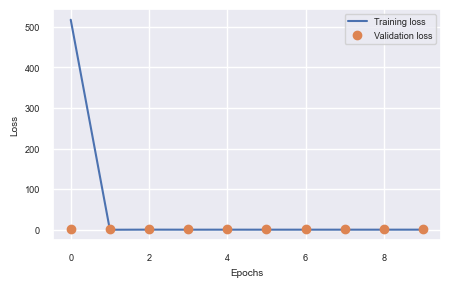
\includegraphics[width=0.7\textwidth]{loss_vs_epochs.png}
\caption{\label{fig:loss_vs_epochs}The training and validation loss for a neural network model trained over 15 epochs with early stopping}
\end{figure}

\begin{lstlisting}[language=Python]
# plotting the training and validation loss
fig, (ax1) = plt.subplots(1, figsize=(5, 3))
ax1.plot(history.history['loss'])
ax1.plot(history.history['val_loss'],'o')
ax1.set_xlabel('Epochs')
ax1.set_ylabel('Loss')
ax1.legend(['Training loss', 'Validation loss'])

plt.show()
\end{lstlisting}

\subsubsection{Model training}

Finally, the model was trained using a similar pipeline, with the optimal combination of parameters and the 8 epochs. The final configuration of this model is visible on Figure \ref{fig:nn_plot}.

\begin{figure}
\centering
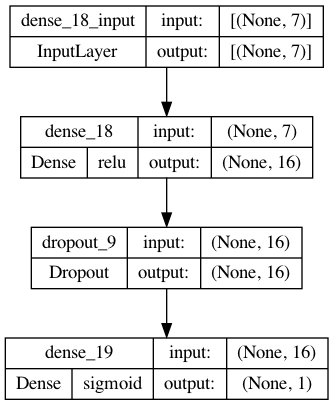
\includegraphics[width=0.35\textwidth]{nn_plot.png}
\caption{\label{fig:nn_plot}The architecture of a neural network model built using Keras}
\end{figure}

\begin{lstlisting}[language=Python]
ann_model = KerasClassifier(
    build_fn=build_clf,
    num_units=grid_search_ann.best_params_['ann_model__num_units'],
    num_hidden_layers=grid_search_ann.best_params_['ann_model__num_hidden_layers'],
    verbose=0
)

ann_pipeline = Pipeline([
    ('scaler', scaler_pipeline), 
    ('ann_model', ann_model)
])

ann_pipeline.fit(
    X_train, 
    y_train,     
    ann_model__epochs=8, 
    ann_model__verbose=0
)
\end{lstlisting}





\subsection{Decision Tree Classifier}
As the data is not linearly separable and it's not possible to find a condition of 100\% correctly classified by a hyperplane, a non-linear classifier is recommended, thus a Decision Tree Classifier was implemented as part of this benchmark.

\subsubsection{Hyperparameter optimisation}
For finding the best parameters for this model, the hyperparameters to tune the model were specified. Then a pipeline was created with 1 step:
\begin{enumerate}
\item \emph{decisiontreeclassifier} which applies the Decision Tree model.
\end{enumerate}

Finally, a grid search was performed using the above-mentioned pipeline and the hyperparameter grid to find the combination with the best accuracy metric with the default cross-validation, that is, a 5-fold cross-validation.
\begin{lstlisting}[language=Python]
tree_pipeline = Pipeline([
    ('decisiontreeclassifier', DecisionTreeClassifier())
])

param_grid = {
    'decisiontreeclassifier__min_samples_split': [2, 5, 10],
    'decisiontreeclassifier__min_samples_leaf': [1, 2, 4],
    'decisiontreeclassifier__max_features': ['sqrt', 'log2']
}

grid_search_tree = GridSearchCV(
    tree_pipeline,
    param_grid=param_grid,
    n_jobs=-1,
    scoring='accuracy',
    verbose=1
)

grid_search_tree.fit(X_train, y_train)
\end{lstlisting}

\subsubsection{Model training}
Then the model was trained using a similar pipeline, but this time with the optimal combination of parameters.

\begin{lstlisting}[language=Python]
tree_pipeline = Pipeline([
    ('decisiontreeclassifier', DecisionTreeClassifier(
        min_samples_split=grid_search_tree.best_params_['decisiontreeclassifier__min_samples_split'],
        min_samples_leaf=grid_search_tree.best_params_['decisiontreeclassifier__min_samples_leaf'],
        max_features=grid_search_tree.best_params_['decisiontreeclassifier__max_features']
    ))
])

tree_pipeline.fit(X_train, y_train)
\end{lstlisting}

\subsection{Random Forest Classifier} 
As the data is not linearly separable and it's not possible to find a condition of 100\% correctly classified by a hyperplane, a non-linear classifier is recommended, thus a Random Forest Classifier was implemented as part of this benchmark.

\subsubsection{Hyperparameter optimisation}
For finding the best parameters for this model, the hyperparameters to tune the model were specified. Then a pipeline was created with 1 step:
\begin{enumerate}
\item \emph{randomforestclassifier} which applies the Random Forest model.
\end{enumerate}

Then, a grid search was performed using the above-mentioned pipeline and the hyperparameter grid to find the combination with the best accuracy metric with the default cross-validation, that is, a 5-fold cross-validation.
\begin{lstlisting}[language=Python]
from sklearn.ensemble import RandomForestClassifier

rf_pipeline = Pipeline([
    ('randomforestclassifier', RandomForestClassifier())
])

param_grid = {
    'randomforestclassifier__class_weight': ['balanced', 'balanced_subsample']
}

grid_search_rf = GridSearchCV(
    rf_pipeline,
    param_grid=param_grid,
    n_jobs=-1,
    scoring='accuracy',
    verbose=1
)

grid_search_rf.fit(X_train, y_train)
\end{lstlisting}

\subsubsection{Model training}
Then the model was trained using a similar pipeline, but this time with the optimal combination of parameters.

\begin{lstlisting}[language=Python]
rf_pipeline = Pipeline([
    ('randomforestclassifier', RandomForestClassifier(
        class_weight=grid_search_rf.best_params_['randomforestclassifier__class_weight']
    ))
])

rf_pipeline.fit(X_train, y_train)
\end{lstlisting}

\section{Evaluation}

\subsection{Classification Report}

The classification reports for all 5 models were generated by the code below.

\begin{lstlisting}[language=Python]
# LinearSVC
cr_linearsvc = metrics.classification_report(y_test, y_predicted_lin_clf, digits=4)

# kNN
cr_knn = metrics.classification_report(y_test, y_predicted_knn, digits=4)

# Neural Networks
y_predicted_ann = y_predicted_ann.flatten()
y_predicted_ann = np.where(y_predicted_ann.round(2) > 0.5, 1, 0)
cr_ann = metrics.classification_report(y_test, y_predicted_ann, digits=4)

# Decision Tree
cr_tree = metrics.classification_report(y_test, y_predicted_tree, digits=4)

# Random Forest
cr_rf = metrics.classification_report(y_test, y_predicted_rf, digits=4)
\end{lstlisting}

\subsubsection{LinearSVC}
\begin{lstlisting}[language=Python]
# printing classification report for LinearSVC
print(cr_linearsvc)
\end{lstlisting}
\begin{verbatim}  
              precision    recall  f1-score   support

           0     0.9980    0.9808    0.9893   2763432
           1     0.7568    0.9687    0.8498    170839

    accuracy                         0.9801   2934271
   macro avg     0.8774    0.9747    0.9195   2934271
weighted avg     0.9840    0.9801    0.9812   2934271
\end{verbatim}

\subsubsection{k-Neighbors Classifier}
\begin{lstlisting}[language=Python]
# printing classification report for kNN classifier
print(cr_knn)
\end{lstlisting}
\begin{verbatim}  
              precision    recall  f1-score   support

           0     0.9999    0.9949    0.9974   2763432
           1     0.9233    0.9979    0.9591    170839

    accuracy                         0.9950   2934271
   macro avg     0.9616    0.9964    0.9782   2934271
weighted avg     0.9954    0.9950    0.9951   2934271
\end{verbatim}

\subsubsection{Neural Networks}
\begin{lstlisting}[language=Python]
# printing classification report for ANN
print(cr_ann)
\end{lstlisting}
\begin{verbatim}    
              precision    recall  f1-score   support

           0     0.9990    0.9857    0.9923   2763432
           1     0.8101    0.9839    0.8885    170839

    accuracy                         0.9856   2934271
   macro avg     0.9045    0.9848    0.9404   2934271
weighted avg     0.9880    0.9856    0.9863   2934271
\end{verbatim}

\subsubsection{Decision Tree}
\begin{lstlisting}[language=Python]
# printing classification report for Decision Tree
print(cr_tree)
\end{lstlisting}
\begin{verbatim}
              precision    recall  f1-score   support

           0     1.0000    0.9998    0.9999   2763432
           1     0.9960    0.9998    0.9979    170839

    accuracy                         0.9998   2934271
   macro avg     0.9980    0.9998    0.9989   2934271
weighted avg     0.9998    0.9998    0.9998   2934271
\end{verbatim}

\subsubsection{Random Forest}
\begin{lstlisting}[language=Python]
# printing classification report for Random Forest
print(cr_rf)
\end{lstlisting}
\begin{verbatim}   
              precision    recall  f1-score   support

           0     1.0000    0.9999    1.0000   2763432
           1     0.9987    1.0000    0.9993    170839

    accuracy                         0.9999   2934271
   macro avg     0.9993    1.0000    0.9996   2934271
weighted avg     0.9999    0.9999    0.9999   2934271
\end{verbatim}


\subsection{Confusion Matrices}
In this section the confusion matrices for every model for test labels were computed and plotted side by side on Figure \ref{fig:confusion_matrices}.

\begin{figure}
\centering
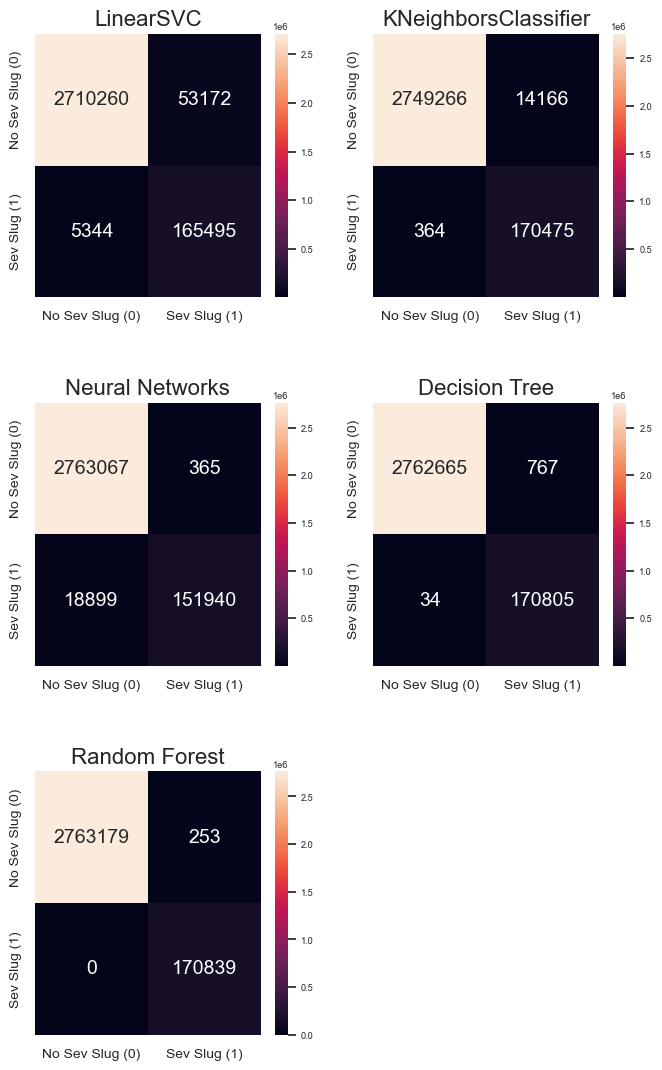
\includegraphics[width=0.75\textwidth]{confusion_matrices.png}
\caption{\label{fig:confusion_matrices}Confusion matrices showing the performance of five machine learning models in predicting severe slugging occurrences}
\end{figure}

\subsection{10-Fold Cross Validation}
Finally, a K-Folds cross-validator was selected to split training data set into 10 consecutive folds and compute the mean accuracy and the respective standard deviation for each model. The models were still put on the same pipelines used on modeling section.

\begin{lstlisting}[language=Python]
models = [    
    ('Random Forest', rf_pipeline), 
    ('Decision Tree', tree_pipeline),
    ('KNeighborsClassifier', knn_pipeline),    
    ('Neural Networks', ann_pipeline), 
    ('Linear SVC', linear_svc_pipeline)
]
\end{lstlisting}
\begin{lstlisting}[language=Python]
for name, model in models:
    kfold = KFold(n_splits=10, shuffle=True, random_state=42)
    
    cv_results = cross_val_score(model, X_train, y_train, cv=kfold, scoring='accuracy')
    cross_validation_dict[name] = cv_results

    msg = "%s: %f (%f)" % (name, np.nanmean(cv_results), np.nanstd(cv_results))
    print(msg)
\end{lstlisting}
\begin{verbatim}
Random Forest: 0.999940 (0.000018)
Decision Tree: 0.999826 (0.000069)
KNeighborsClassifier: 0.998610 (0.000138)
Neural Networks: 0.978187 (0.001739)
Linear SVC: 0.974343 (0.000403)
\end{verbatim}

The following code was implemented to plot how the mean score after cross validation was distributed in each model. This chart can be visualised on Figure \ref{fig:10_fold_cv}.

\begin{lstlisting}[language=Python]
# comparing algorithms
fig = plt.figure()
fig.suptitle('Distribution of Mean Score After 10-fold Cross Validation By Algorithm')
ax = fig.add_subplot(111)
plt.boxplot(cross_validation_dict.values())
ax.set_xticklabels(cross_validation_dict.keys())
fig.set_size_inches(8,4)
plt.show()
\end{lstlisting}

\begin{figure}
\centering
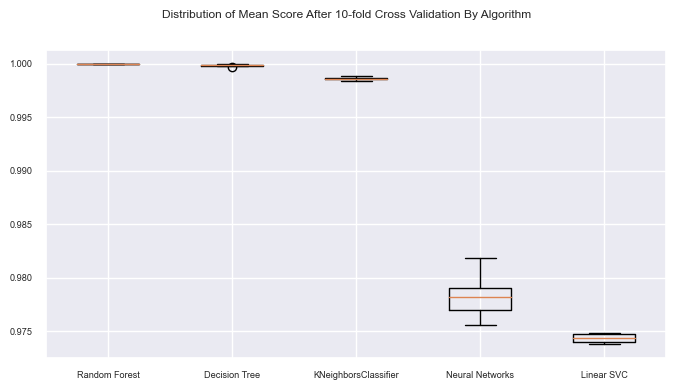
\includegraphics[width=0.75\textwidth]{10_fold_cv.png}
\caption{\label{fig:10_fold_cv}Box plots showing the distribution of Mean Score After 10-fold Cross Validation By Algorithm}
\end{figure}.


\section{Conclusion}

In this study, Random Forest and Decision Tree Classifiers had the best performance overall with 99.994\% and 99.982\% of accuracy respectively. These non-linear classifiers could find better results because the 3W data set does not present a clear linear separability between records related to Severe Slugging and other normal records or other undesirable events.



\iffalse

% \subsection{How to write Mathematics}

% \LaTeX{} is great at typesetting mathematics. Let $X_1, X_2, \ldots, X_n$ be a sequence of independent and identically distributed random variables with $\text{E}[X_i] = \mu$ and $\text{Var}[X_i] = \sigma^2 < \infty$, and let
% \[S_n = \frac{X_1 + X_2 + \cdots + X_n}{n}
%       = \frac{1}{n}\sum_{i}^{n} X_i\]
%  denote their mean. Then as $n$ approaches infinity, the random variables $\sqrt{n}(S_n - \mu)$ converge in distribution to a normal $\mathcal{N}(0, \sigma^2)$.


\fi

\printbibliography

\end{document}